\documentclass[a4paper,12pt,reqno]{article}

\newcommand{\titl}{NumMeth MAT-410 Lab 3 Report}
\newcommand{\auth}{Moritz M. Konarski}
\usepackage{amsmath}
\usepackage{amssymb}
\usepackage[margin=1in]{geometry}
\usepackage[english]{babel}
\usepackage[pdftitle={\titl},pdfauthor={\auth},final]{hyperref}
\usepackage{graphicx}
\usepackage{mathptmx}
\usepackage[T1]{fontenc}
\usepackage{accents}
\usepackage{float}
\newcommand{\figref}[1]{Figure~\ref{#1}}
\newcommand{\tabref}[1]{Table~\ref{#1}}
\renewcommand{\baselinestretch}{1.2}
\setcounter{tocdepth}{2}
\usepackage{accents}
\usepackage[document]{ragged2e}

\setlength{\RaggedRightParindent}{0.25in}

\title{\titl}
\author{\auth}
\date{\today}

\begin{document}
\maketitle
\tableofcontents

\section{Introduction}

\noindent
The third laboratory project of this course deals with two--dimensional Poisson
equation (also called Dirichlet equations). We consider these equations on the
unit square $\Omega$, defined as follows
\begin{equation}\nonumber
    \Omega = \{(x,y) | 0 \le x \le 1, 0 \le y \le 1 \}.
\end{equation}
\noindent
The borders of this unit square are defined as $\partial \Omega$
\begin{equation}\nonumber
    \begin{gathered}
        \partial \Omega = \{ x = 0, 0 \le y \le 1 \} \cup 
        \{ x = 1, 0 \le y \le 1\} \cup \\
        \{0 \le x \le 1 , y = 0\} \cup 
        \{0 \le x \le 1, y = 1 \}.
    \end{gathered}
\end{equation}
\noindent
The Poisson equations describes a thermal field whose source is the function
$f(x,y)$, and the operator $\Delta$ is the Laplace Operator, as seen below.

\begin{equation}\nonumber
    \begin{gathered}
        - \Delta u(x,y) \equiv - \left(\frac{\partial^2 u}{\partial x^2} 
            + \frac{\partial^2 u}{\partial y^2} \right) = f(x,y), 
            \quad (x,y) \in \stackrel{0}{\Omega}
        \equiv \Omega \backslash \partial \Omega    \\
        u(x,y) = 0, \quad (x,y) \in \partial \Omega
    \end{gathered}
\end{equation}
To solve this equation we consider a uniform two--dimensional grid called
$\Omega^h$. On this grid we have the function 
\begin{equation}\nonumber
    \bar u^h_{i,j},
\end{equation}
which represents the numerical solution on $\Omega^h$. The variables $(i,j)$ here
are the indices of the grid, where $x_i = i \cdot h$ and $y_j = j \cdot h$ ($h$
is the step size). The function $f(x,y)$ is now written as $f_{i,j}$.
This report uses a point--wise form of the finite--difference solution. By
iterating this method multiple times, a desired accuracy of the approximation
can be reached. Here $k$ is the iteration parameter. For each point
$u^{(k)}_{i,j}$ we have
\begin{equation}\label{eq:it}
    \begin{gathered}
        u^{(k)}_{i,j} = 
        \frac{\theta}{4}\left( u^{(k)}_{i-1,j} + u^{(k)}_{i,j-1} \right)
    + \frac{\tau-\theta}{4}\left( u^{(k-1)}_{i-1,j} + u^{(k-1)}_{i,j-1}
            \right) \\
    + \frac{\tau}{4}\left( u^{(k-1)}_{i+1,j} + u^{(k-1)}_{i,j+1} \right)
    + (1-\tau) u^{(k-1)}_{i,j} + \frac{\tau h^2}{4}\cdot f^h; \quad (i,j) \in
    \Omega^{h,0}    \\
        u^{(k)}_{i,j} = 0, \quad (i,j) \in \partial \Omega^h
    \end{gathered}
\end{equation}

The parameters $\tau$ and $\theta$ as well as the function $f_{i,j}$ are 
determined by the methods or the task, respectively. Equation \eqref{eq:it} 
is used in an iteration over all steps in $x$ for each of the levels in
$y$. Thus equation \eqref{eq:it} approximates the Poisson equations using repeated
iteration for each point in $\Omega^{h,0}$, the inner part of the uniform grid.\\

\subsection{The Task}

This report specifically covers the eigenfunctions of the grid Laplace operator
$\Delta^h$. According to my readme file, I should choose the parameters $l$ and
$m$ to be 2. Accordingly, the analytic solution in the unit--square $\Omega$ is
defined as 
\begin{equation}\label{eq:an}
    u^h_{i,j} = \sin(2\pi x_i) \cdot \sin(2\pi y_j).
\end{equation}
The function $f_{i,j}$ is defined as
\begin{equation}\nonumber
    \begin{gathered}
        f^h_{i,j} = \lambda_{2,2} - \sin(2\pi x_i) \cdot \sin(2\pi y_j) \\
        \lambda_{2,2} = \frac{4}{h^2} 
            \cdot \left[ \sin^2\left(\frac{2\pi h}{2}\right) 
            + \sin^2\left(\frac{2\pi h}{2}\right) \right]
    \end{gathered}
\end{equation}
for the values $l=2$ and $m=2$. It has to be noted that because $l=m$ the error
of the approximation for the $x$ and $y$ slices is identical and thus they do
not need to be differentiated.

\subsection{The Methods}

The methods used to solve the Poisson equations through iteration are Jacobi's 
method and Seidel's method. For Jacobi's method, the parameters $\tau$ and
$\theta$ are chosen as $\tau = 1$ and $\theta = 0$.
For Seidel's method, $\tau = 1$ and $\theta = 1$. These parameters influence 
the behavior of the point--wise iterative function in \eqref{eq:it} and lead to 
different processes of approximation.\\
In my program the user chooses an error threshold $\sigma$ that, when the error 
is lower than it, stops the iterative process. This will halt the program at 
the minimum required number of iterations to satisfy the error threshold.\\
In the following sections I will compare the speed of convergence for both
methods based on the number of grid nodes, their convergence based on the
values of the parameters $l$ and $m$ (different from the ones I was given), and 
the effectiveness of the methods as measured by the number of required 
iterations to achieve a predetermined accuracy $\sigma$, the errors of each 
method, and the visual proximity of the graph of the numerical solution to the
analytic solution.

\section{Speed of Convergence}

The speed of convergence for both methods strongly depends on the parameter
$n$, the number of grid nodes. The higher the number of grid nodes is, the more
iterations are required to reach the error threshold $\sigma$. I think the 
reason for this is that for each new grid node, additional computation (and 
iteration) is required to approximate its correct position. Increased numbers 
of grid nodes will also increase the overall accuracy of the approximation 
because more nodes allow a more fine--grained fit of the numerical solution to
the analytical solution.\newline
In \figref{n_jacobi} (left graph) we can see that the number of required 
iterations to reach an error threshold of $\sigma=0.001$ drastically increases 
as the number of nodes increases. This is not just caused by this particular 
error threshold, the graph on the right shows the same behavior for a much 
smaller error threshold of $\sigma=0.00001$.
Through \figref{n_jacobi} we can also note that the number of required 
iterations increases as the error threshold decreases -- this will be covered 
in more detail later.
\begin{figure}[H]
    \center
    \fbox{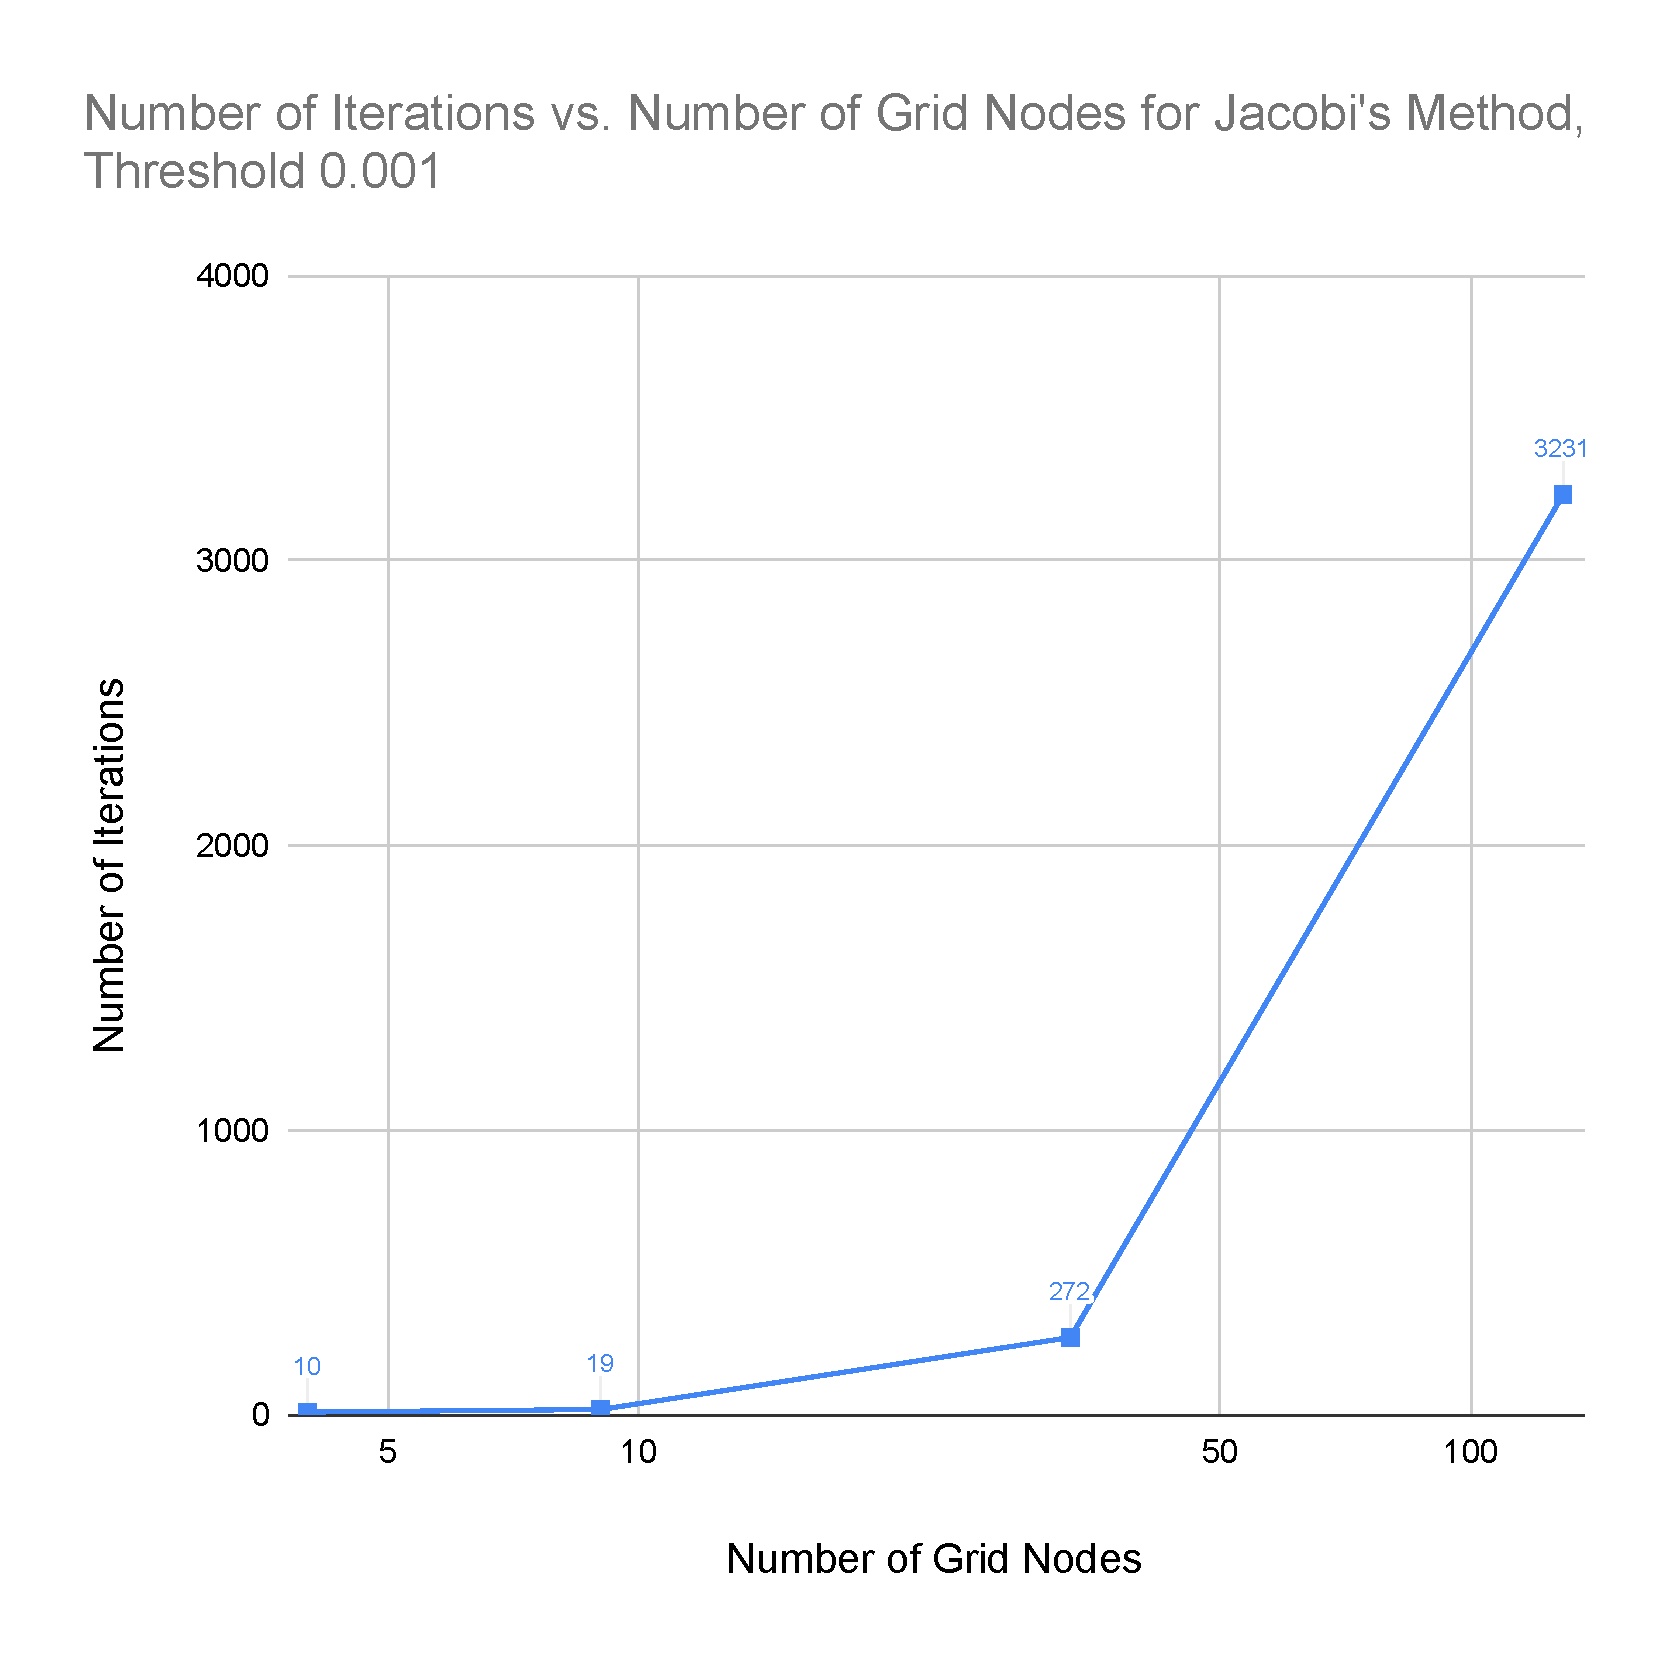
\includegraphics[width=0.45\textwidth]{../graphs/chart}}
    \hspace{3pt}
    \fbox{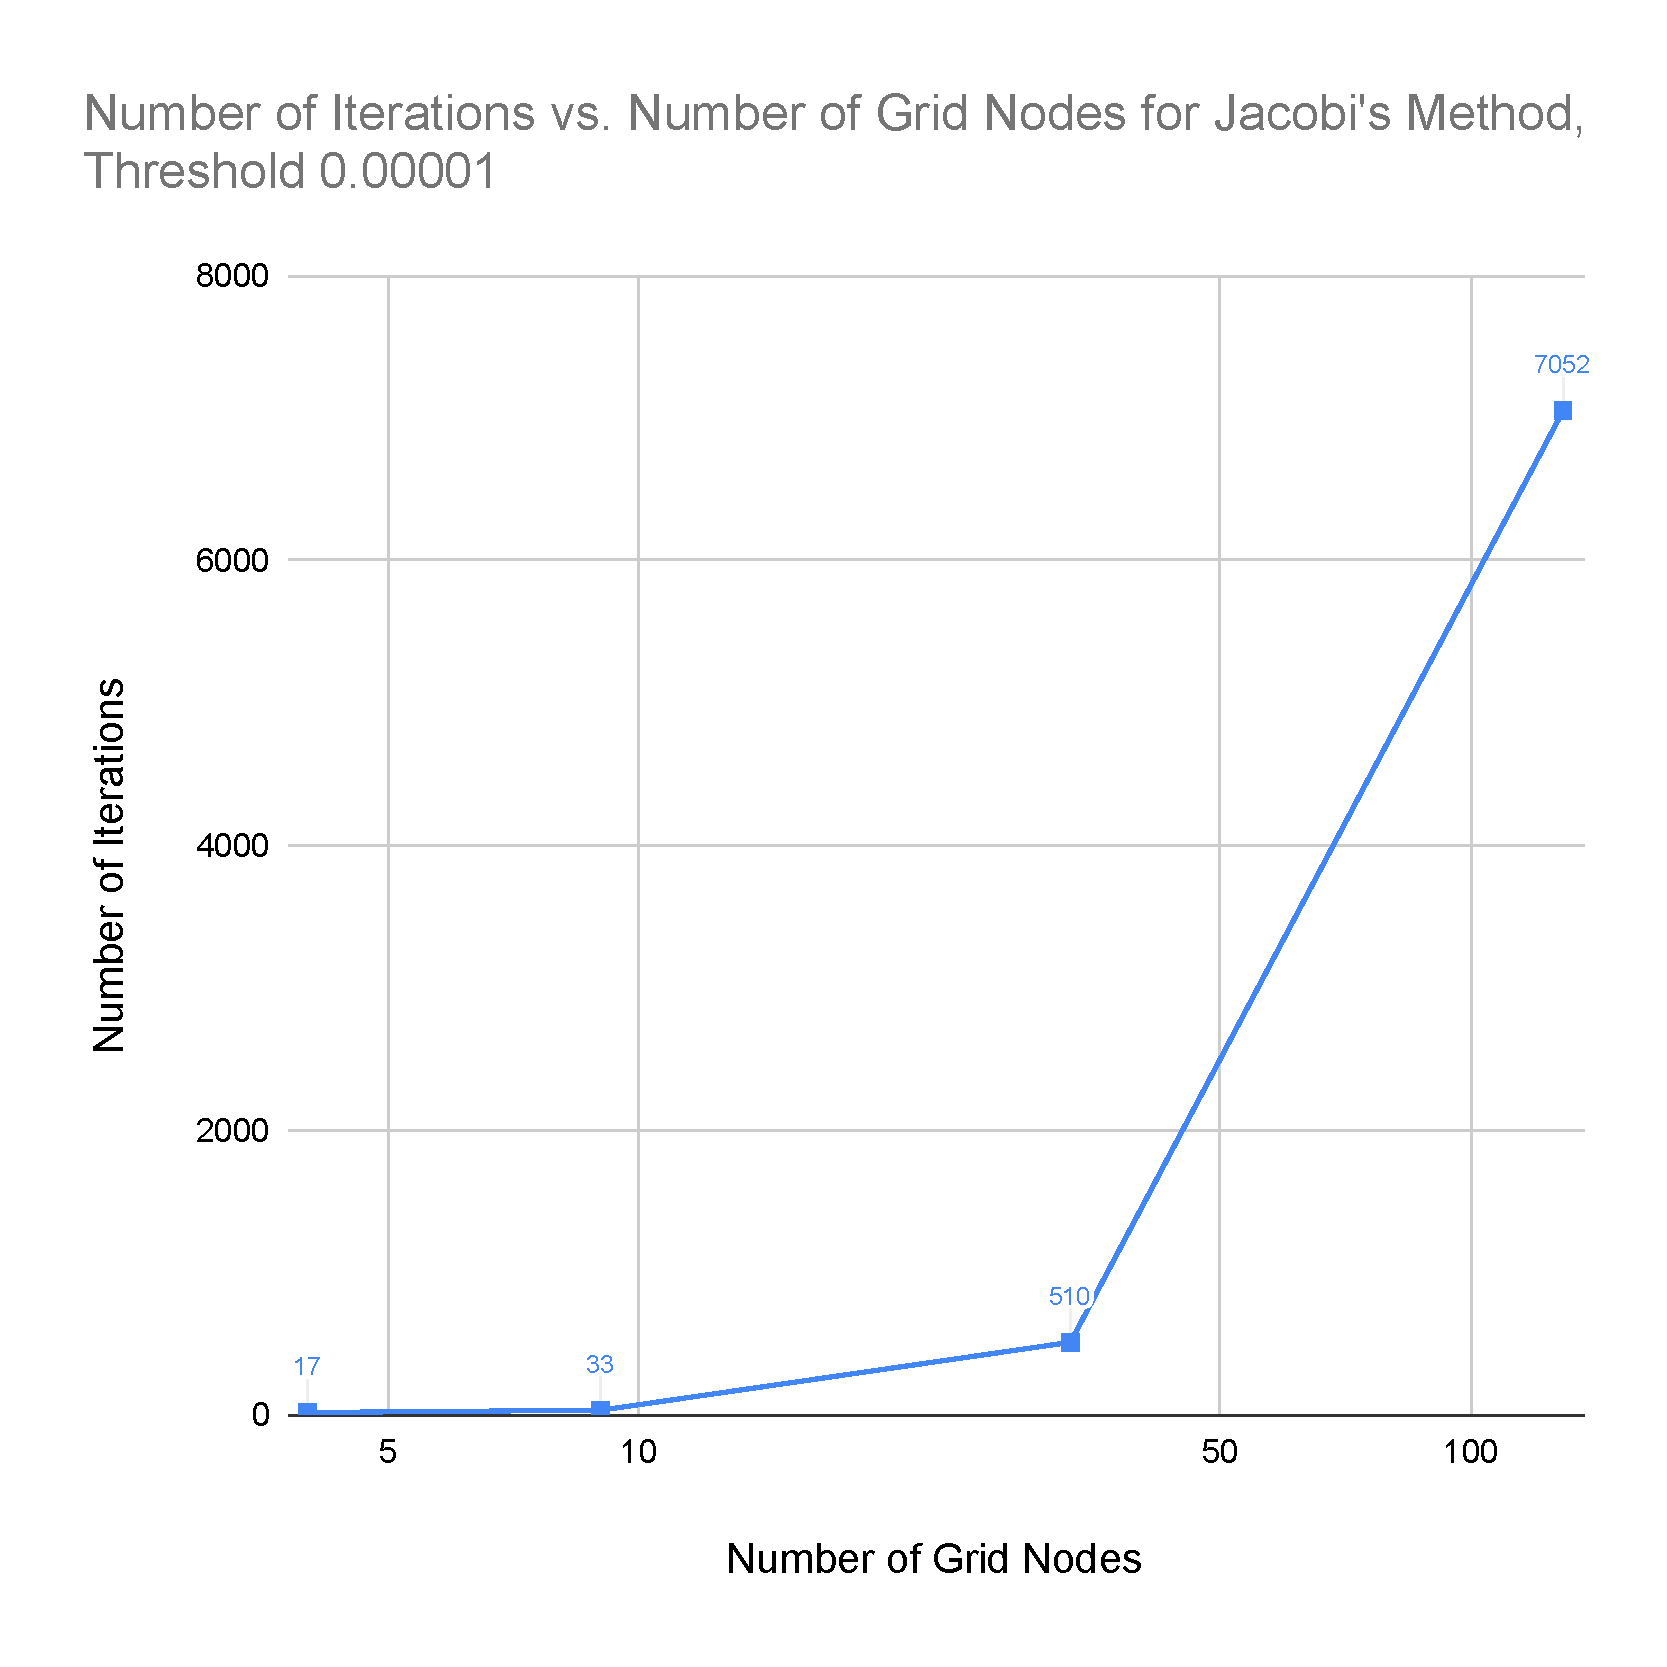
\includegraphics[width=0.45\textwidth]{../graphs/chart (3)}}
    \caption{Iterations for Jacobi's Method, $\sigma=0.001$ and $\sigma=0.00001$}
    \label{n_jacobi}
\end{figure}

When considering Seidel's method, much the same behavior from Jacobi's method 
is evident.
\figref{n_seidel} (left graph) shows the required iterations of Seidel's
method for a 
threshold of $\sigma=0.001$ as the number of grid nodes increases. 
The right graph shows the required iterations for a threshold of
$\sigma=0.00001$.
\begin{figure}[H]
    \center
    \fbox{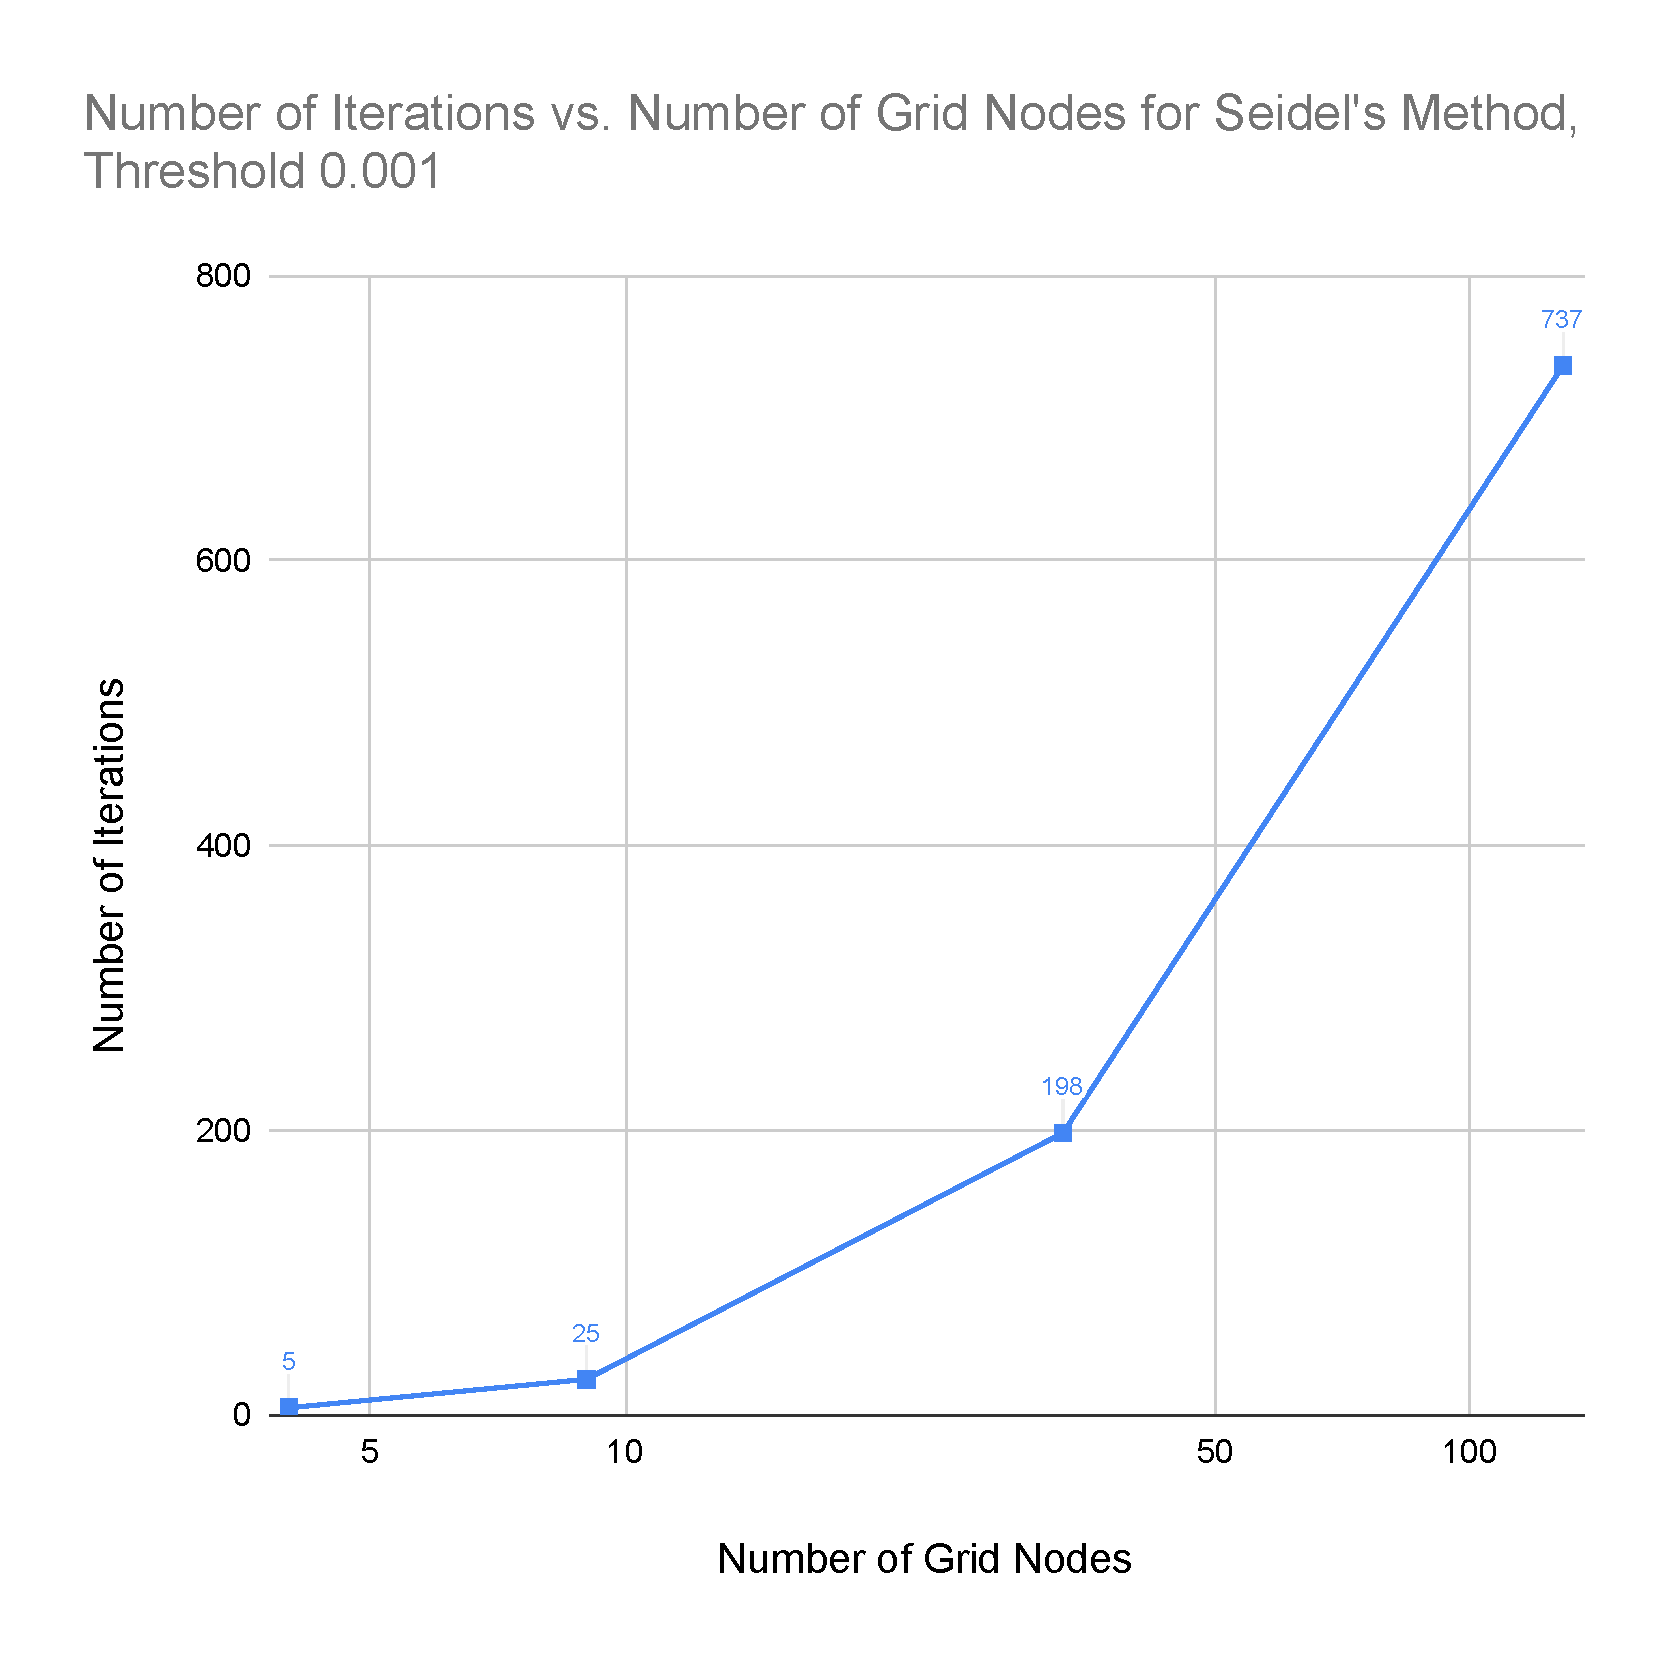
\includegraphics[width=0.45\textwidth]{../graphs/chart (4)}}
    \hspace{3pt}
    \fbox{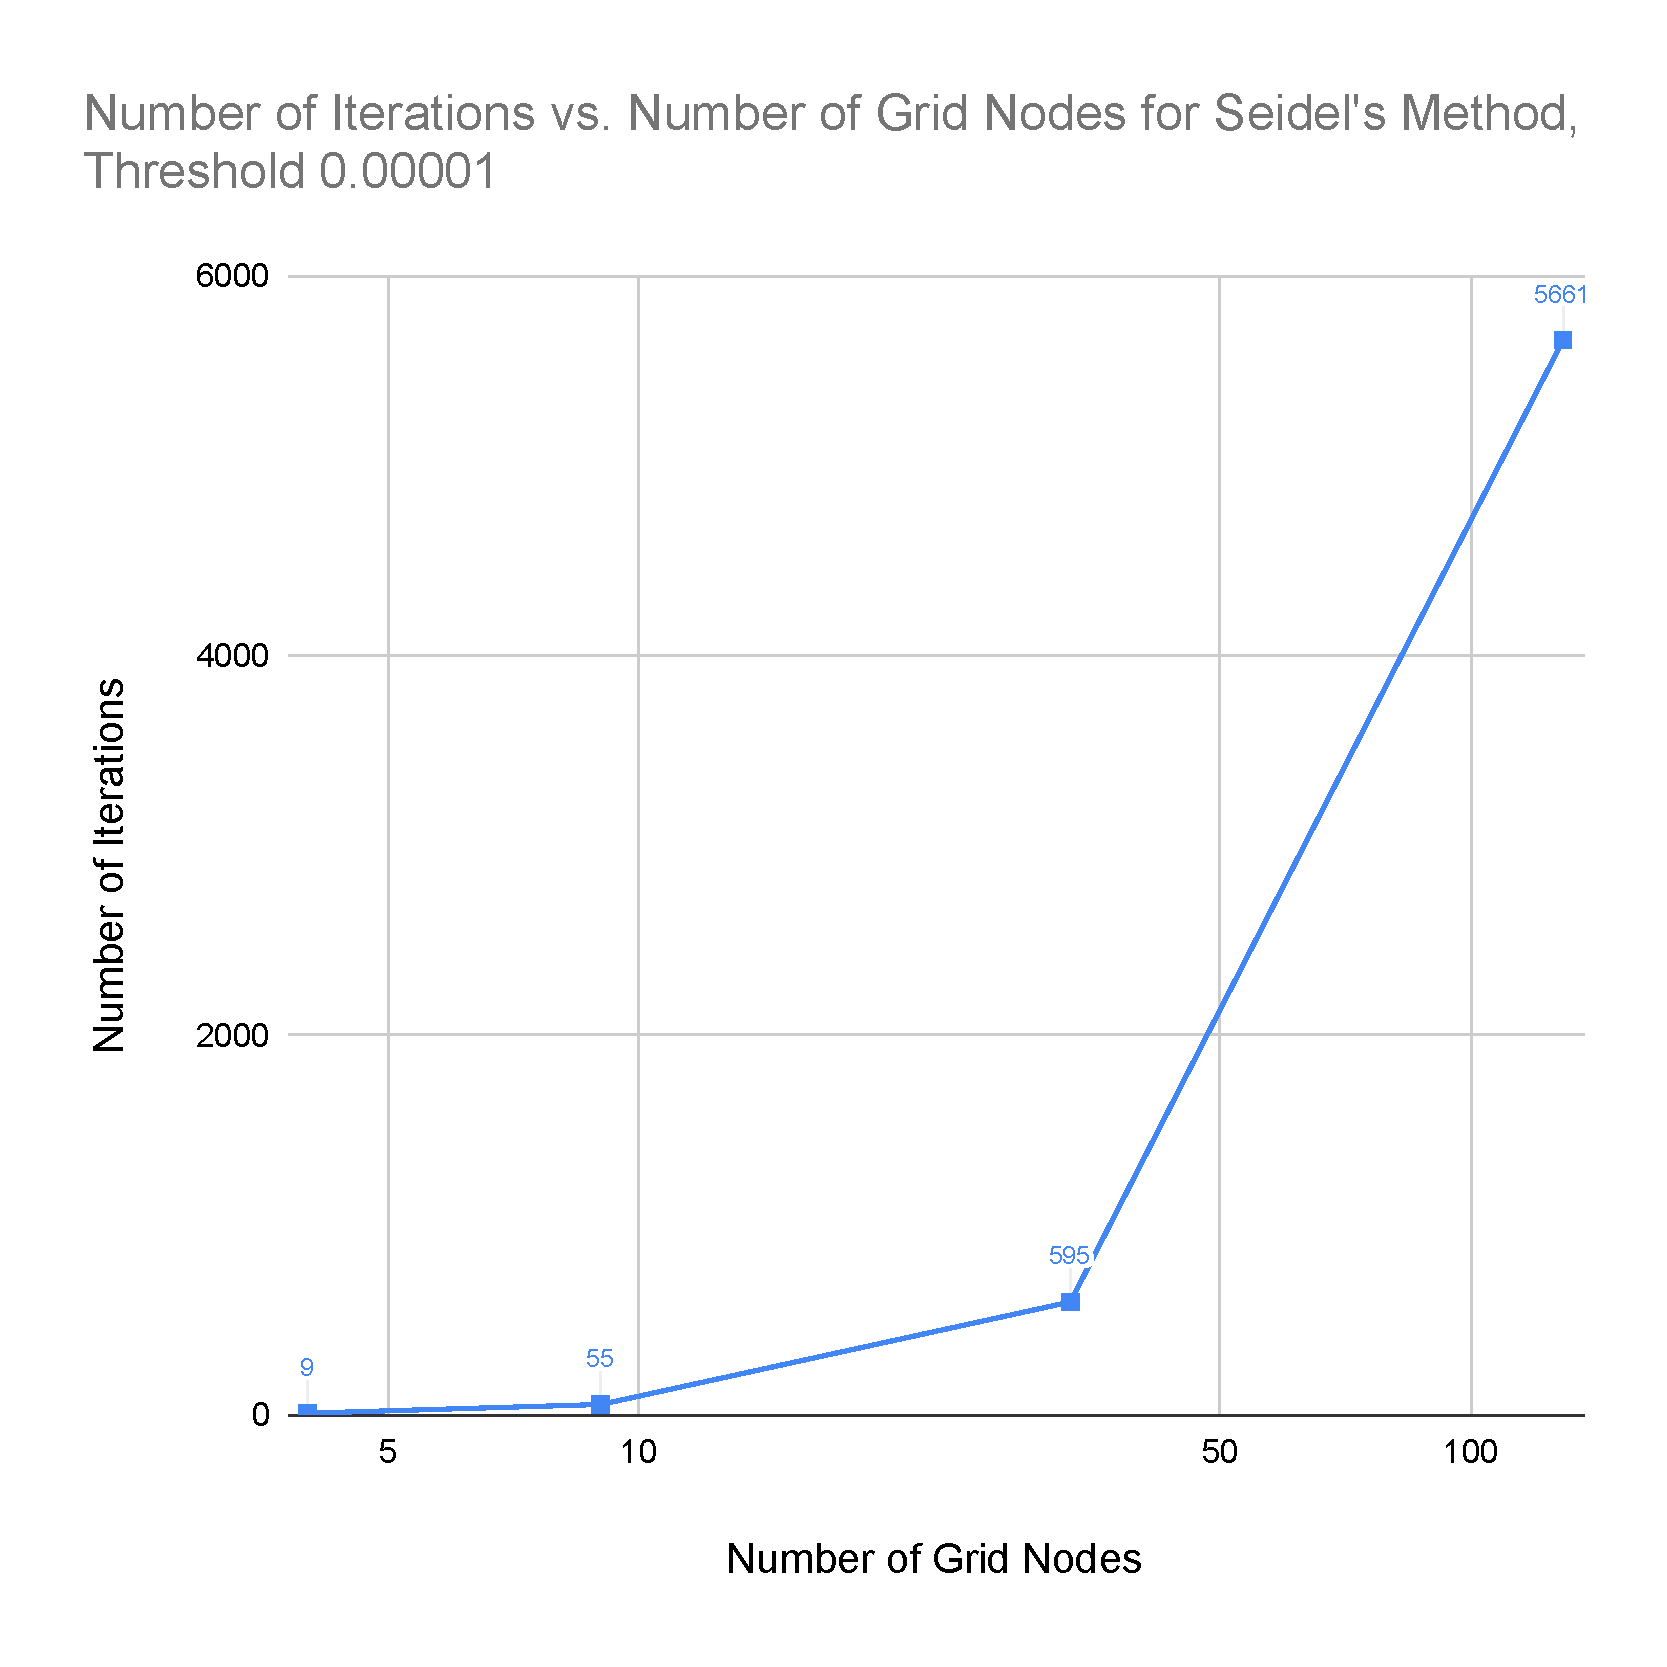
\includegraphics[width=0.45\textwidth]{../graphs/chart (5)}}
    \caption{Iterations for Seidel's Method, $\sigma=0.001$ and $\sigma=0.00001$}
    \label{n_seidel}
\end{figure}

\section{Complexity of the Solutions}

The parameters $l$ and $m$ determine how many periods of the sine functions in 
equation \eqref{eq:an} exist on the interval $[0,1]$. The parameter $l$
influences the periods in the $x$ dimension and $m$ the periods in the $y$
dimensions. For multiples of 2 one full period exists. For my values of 
$l=m=2$, one
full period of the sine wave exists on the interval $[0,1]$ in both the $x$ and
$y$ dimensions.\\
The values of these parameters influence the number of iterations required to 
reach a certain error threshold. Unfortunately, I was not able to determine
exactly in what way. In one case, decreasing $l$ to 1 and increasing $m$ to
3 increased the number of required iterations. This can be seen in
\figref{fig:complex} looking at the red graph.
In another case, increasing $l$ to 10 and increasing $m$ to 4 dramatically
decreased the number of required iterations. This behavior can be see in the
yellow graph in \figref{fig:complex}. The blue graph shows the required
iterations for $l = m = 2$ for reference.\\
I could not find a correlation between the values of $l$ and $m$ and the number
of required iterations to achieve an error below $\sigma=0.0001$. The only 
thing this shows is that the required iterations change dependent on the 
values of $l$ and $m$.
\begin{figure}[H]
    \center
    \fbox{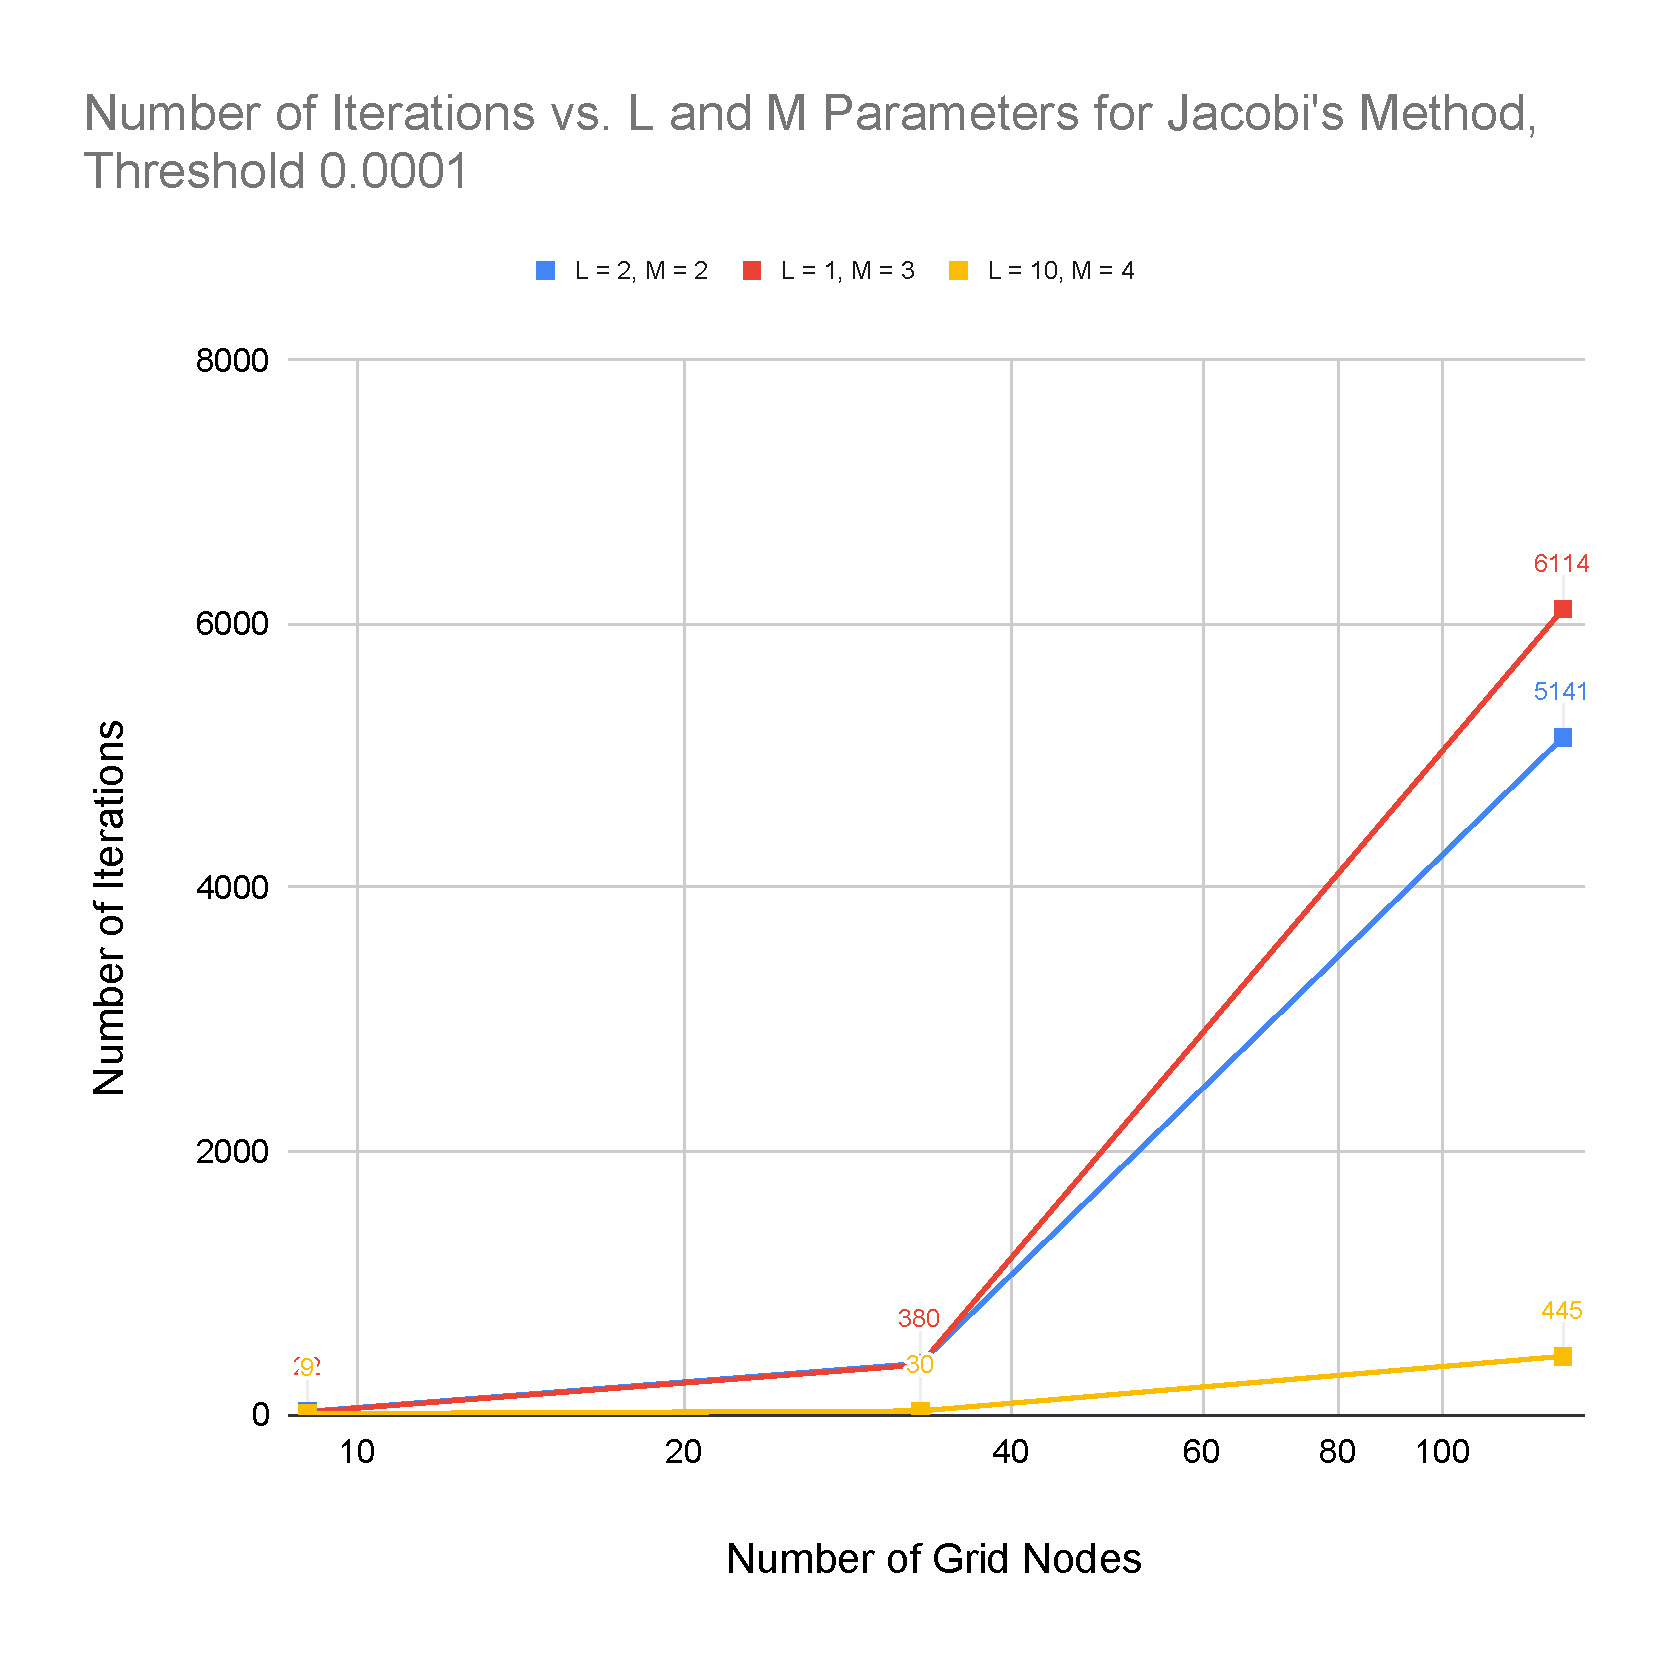
\includegraphics[width=0.45\textwidth]{../graphs/chart (1)}}
    \hspace{3pt}
    \fbox{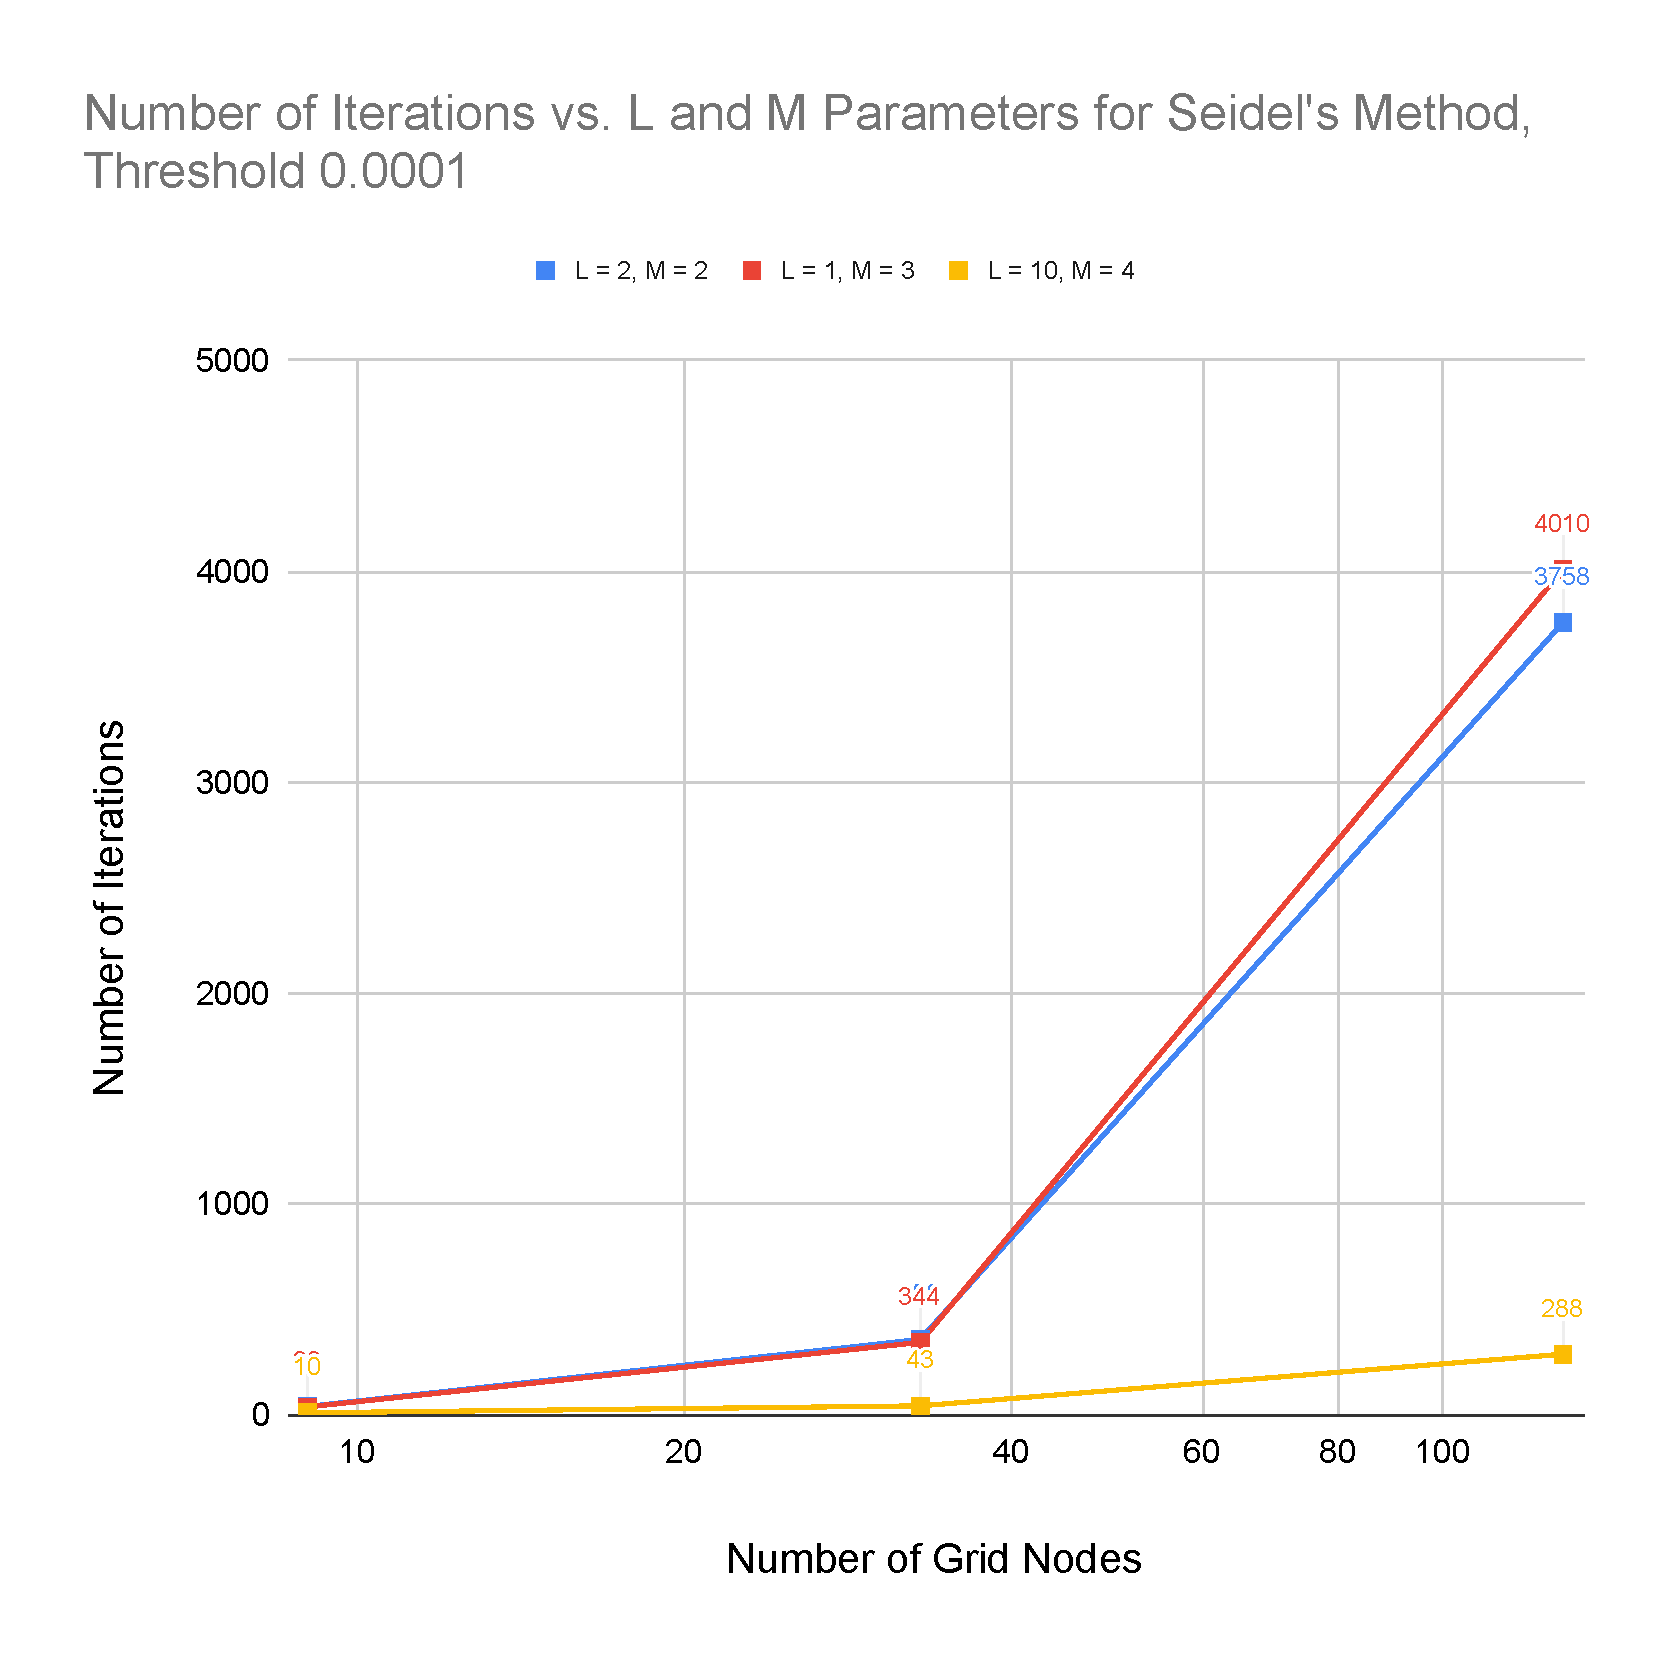
\includegraphics[width=0.45\textwidth]{../graphs/chart (2)}}
    \caption{Iterations for Jacobi's and Seidel's Method, $\sigma=0.0001$,
    varying $l$ and $m$}
    \label{fig:complex}
\end{figure}

\section{Effectiveness of the Methods}

This section will evaluate the effectiveness of the methods as measured by the 
number of required iterations to achieve a predetermined accuracy $\sigma$, the 
errors of each method, and the visual proximity of the graph of the numerical 
solution to the analytic solution.

\subsection{Number of Required Iterations}

My analysis of the number of required iterations to reach a certain error
threshold $\sigma$ was inconclusive. For certain combinations of $\sigma$ and
$n$ Jacobi's method requires fewer iterations than Seidel's method while for
other combinations it is the other way around.\\
Nonetheless, for the majority of combinations Seidel's method required fewer
iterations to reach the error threshold. In \figref{fig:complex} we can see
that the highest numbers of iterations for $\sigma=0.0001$ and $n=129$ for 
Jacobi's method are $5141, 6114, 445$, while for Seidel's method the errors for 
the same combination are $3758, 4010, 288$. All errors for Seidel's method here 
are smaller than the ones for Jacobi's method.\\
Furthermore, comparing two of the previous figures for $\sigma=0.00001$ in
\figref{fig:its} for Jacobi's method and Seidel's method shows that for
$n=4,9,33$ Jacobi's method requires fewer iterations than Seidel's method. When
$n=129$, Seidel's method requires fewer iterations than Jacobi's method. This
is one example of how one of the methods is better than the other and then that
changes when $n$ increases.
\begin{figure}[H]
    \center
    \fbox{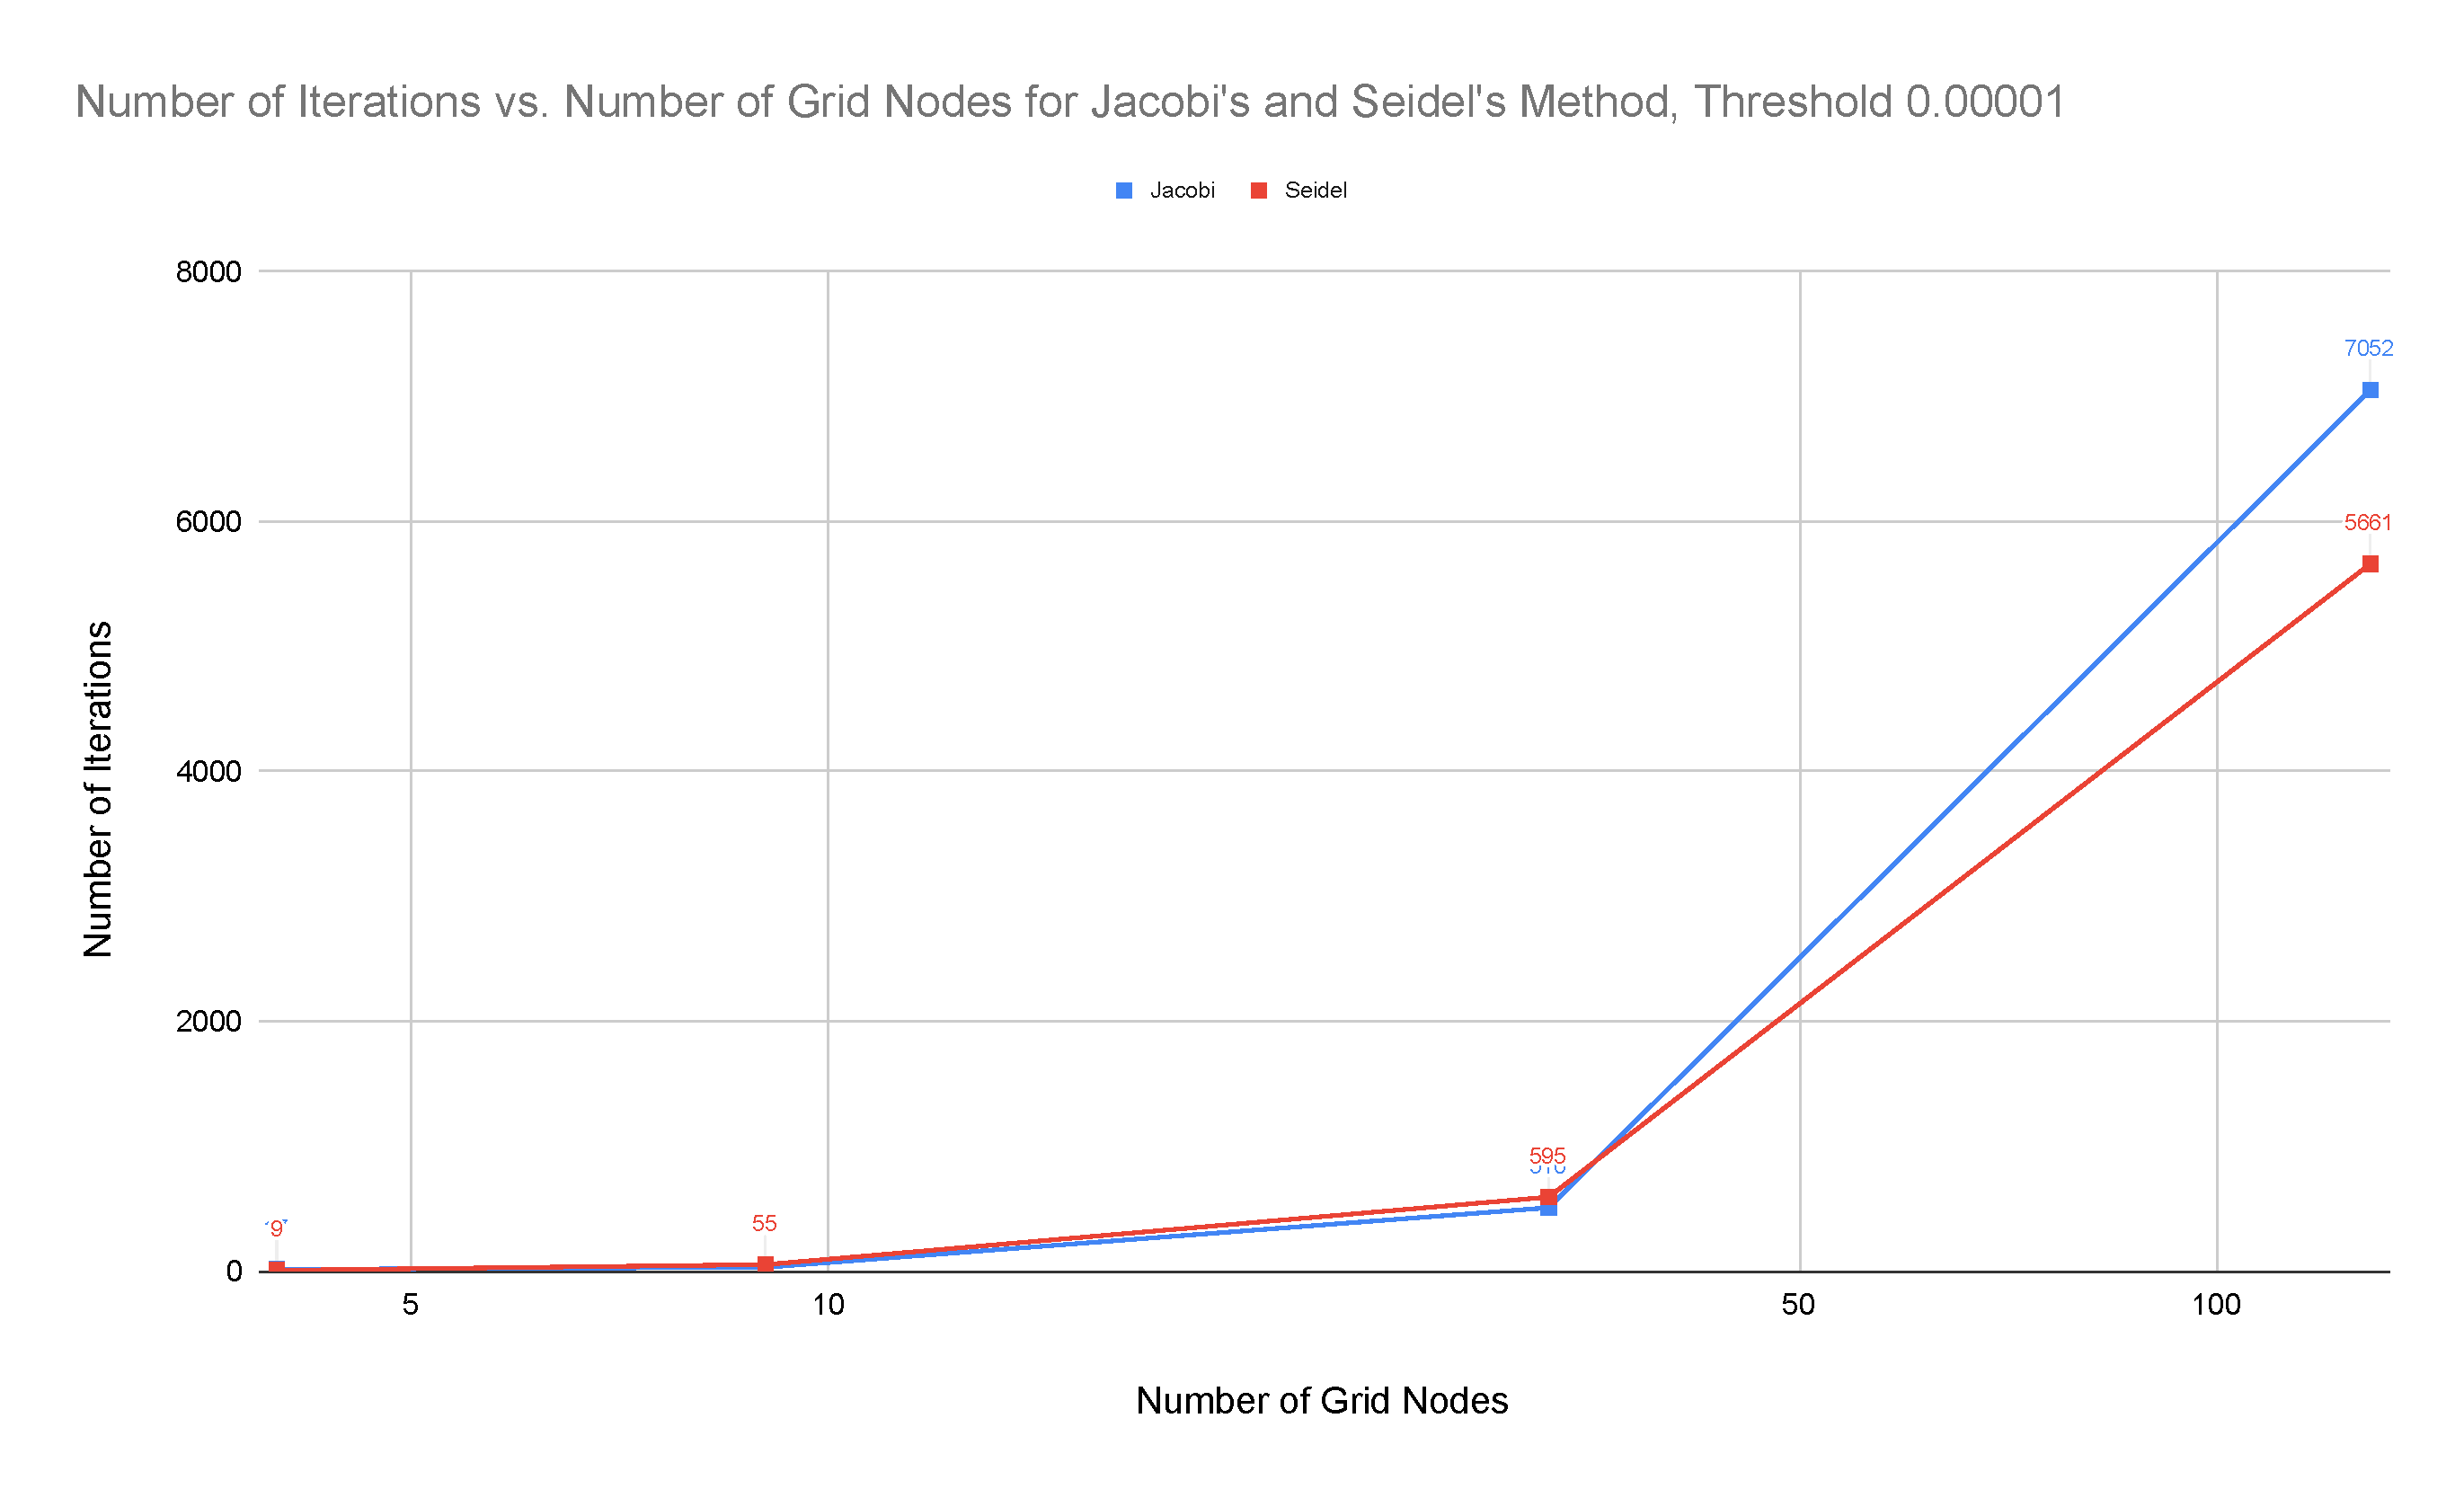
\includegraphics[width=0.8\textwidth]{../graphs/iteration}}
    \caption{Iterations for Jacobi's and Seidel's Method, $\sigma=0.00001$}
    \label{fig:its}
\end{figure}

\subsection{Errors}

Both methods converge to the analytic solution and thus the actual solution.
Out of the two methods, Seidel's method converges much faster than Jacobi's
method at first. After that, the error of its approximation increases again,
before approaching the error threshold again. Jacobi's method has no such
quirks and steadily decreases its error with each iteration. \figref{fig:err}
shows this behavior. Please note that the error is displayed on a logarithmic
scale with base 10.
\begin{figure}[H]
    \center
    \fbox{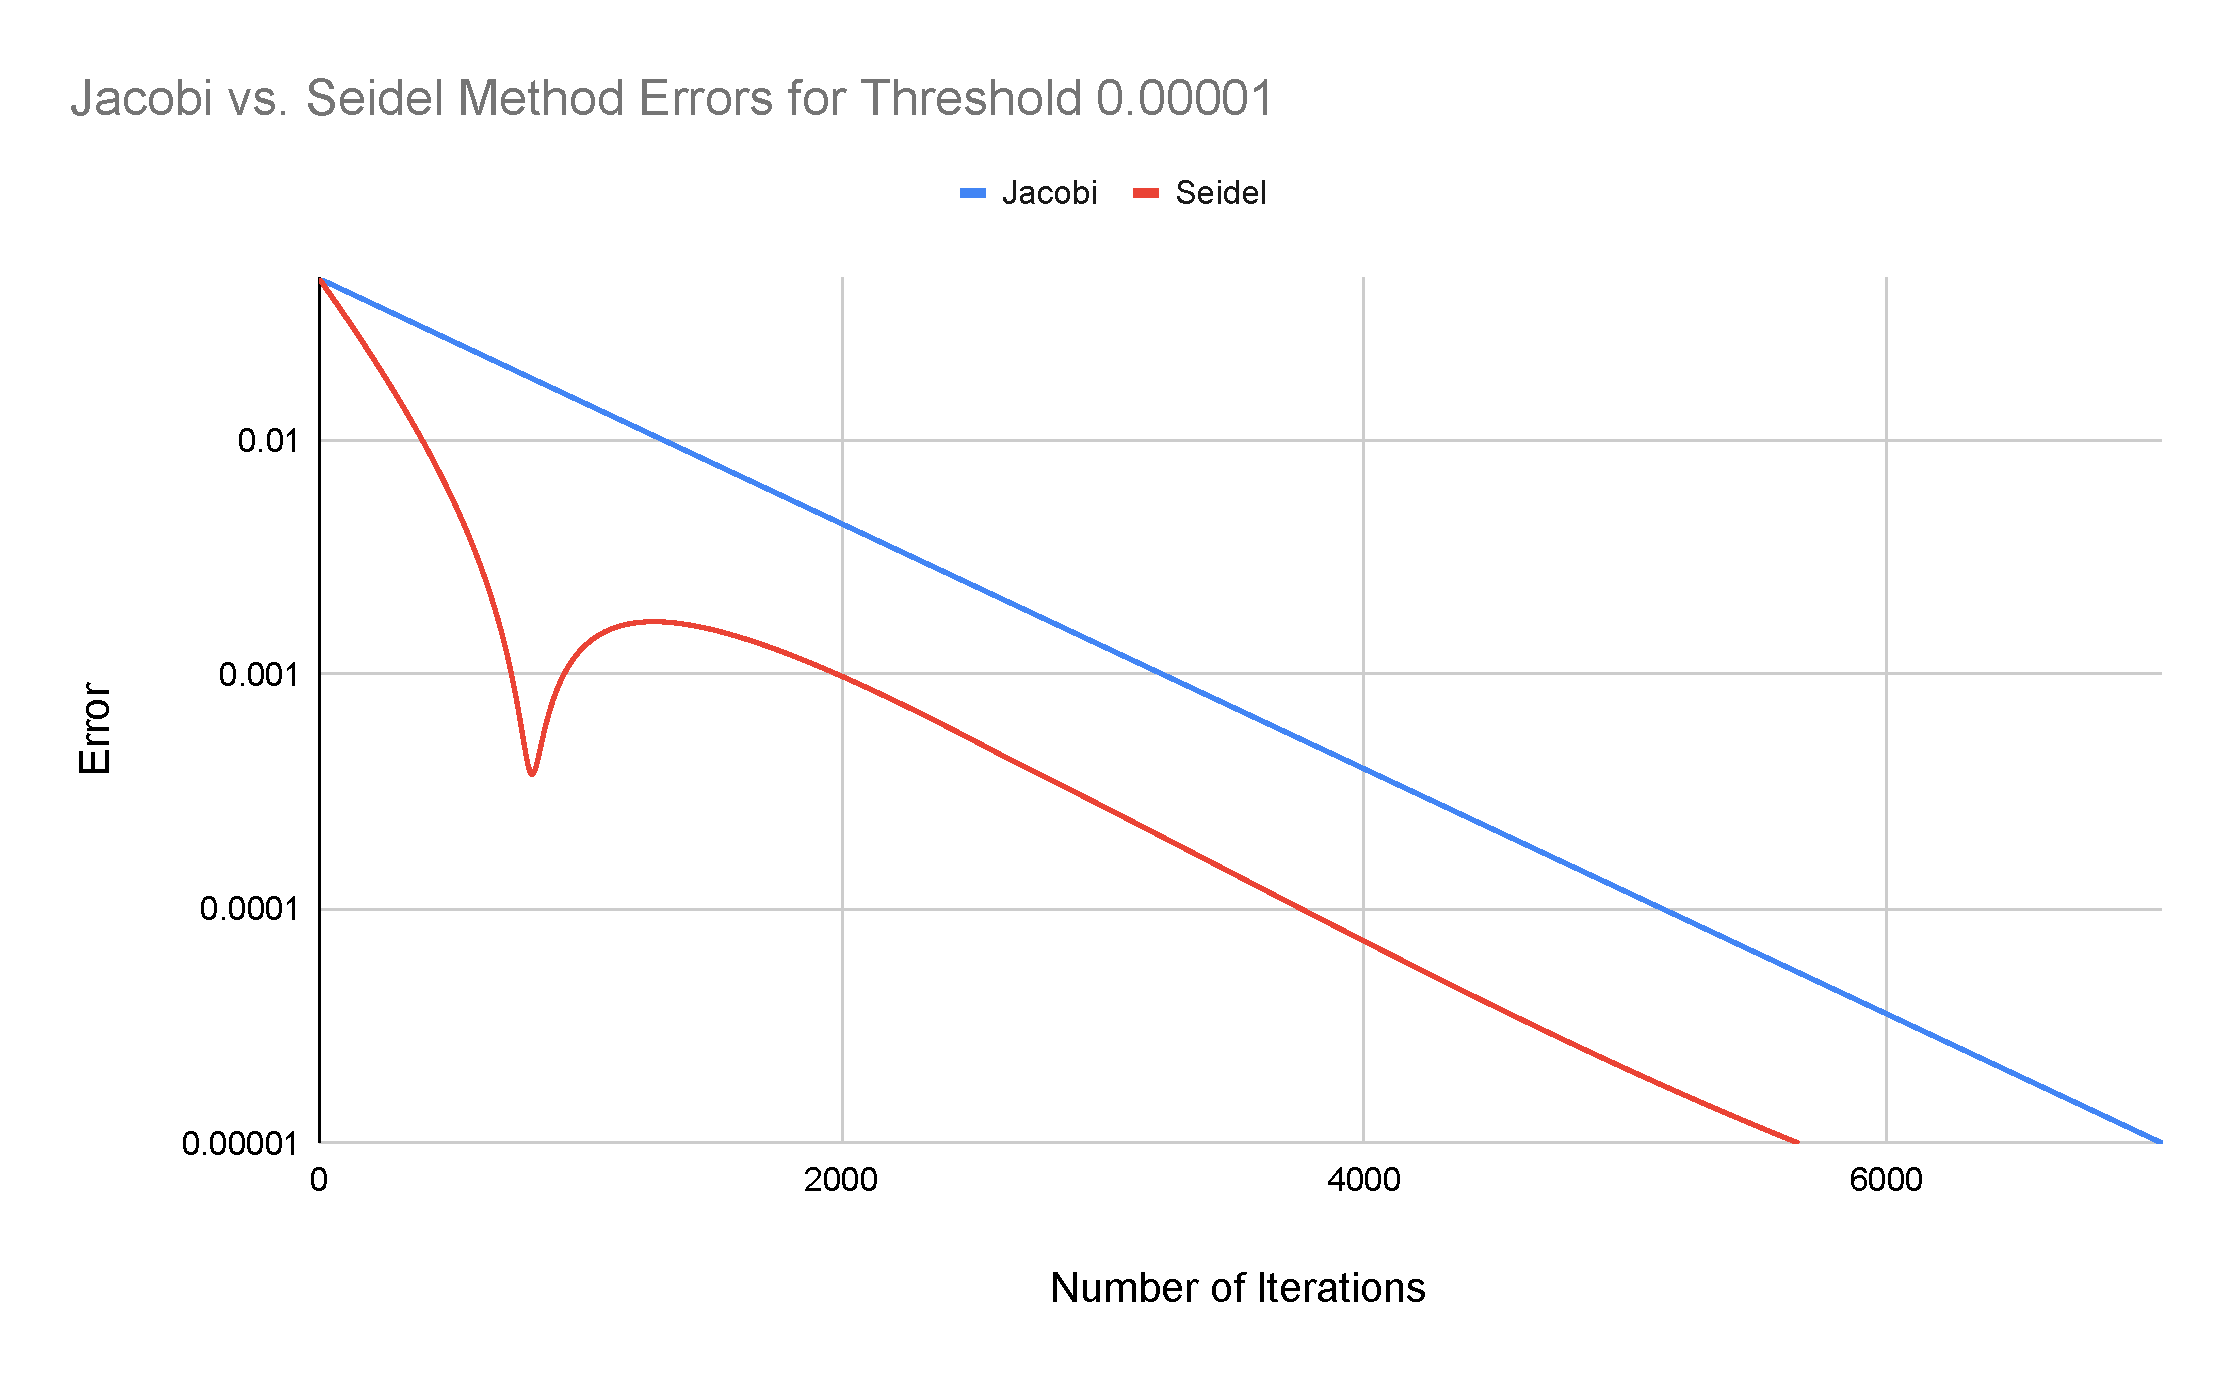
\includegraphics[width=0.8\textwidth]{../graphs/errors}}
    \caption{Error for Jacobi's and Seidel's Method, $\sigma=0.00001$, $n=129$}
    \label{fig:err}
\end{figure}

\subsection{Visual Proximity of the graphs}

In this comparison Seidel's method clearly is the winner. Because of the rapid
convergence shown in \figref{fig:err}, the numerical solution quickly comes 
close enough to the analytic solution that they look identical. This does not
necessarily mean that the error threshold is reached more quickly, but it looks
like it. In \figref{fig:vis1} we can see that for $n=129$ at 250 iterations, 
Seidel's method (on the right) has already converged much close to the analytic 
solution than Jacobi's method (on the left).
\begin{figure}[H]
    \center
    \fbox{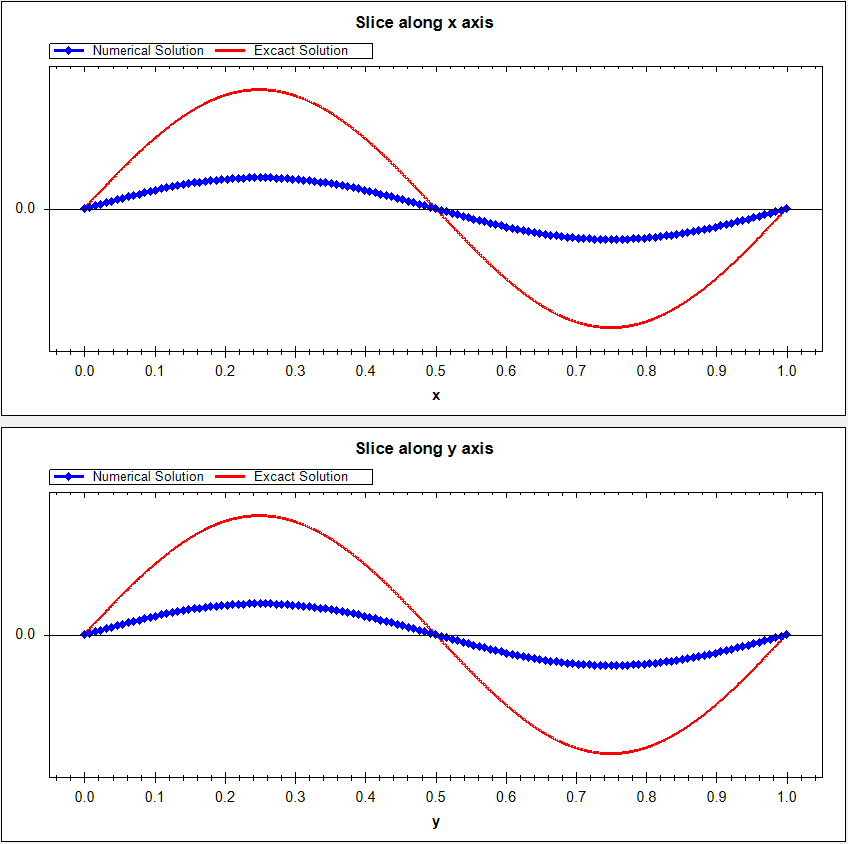
\includegraphics[width=0.45\textwidth]{../graphs/jacobi_129_0.001_250}}
    \hspace{3pt}
    \fbox{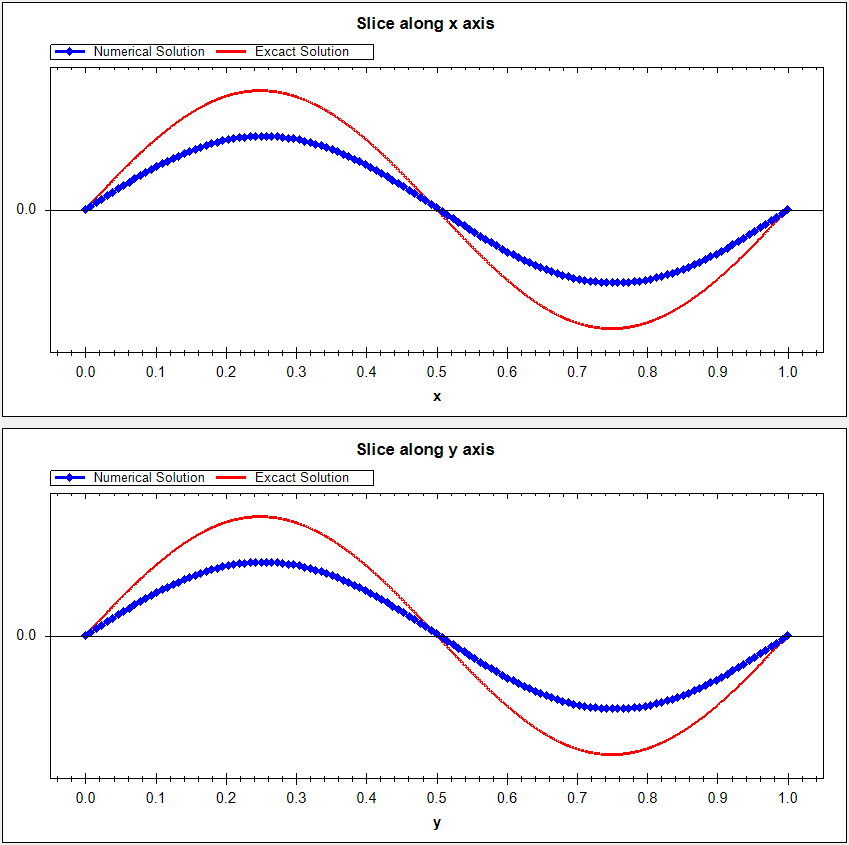
\includegraphics[width=0.45\textwidth]{../graphs/seidel_129_0.001_250}}
    \caption{Visual comparison of Jacobi and Seidel method graphs for $n=129$,
    250th iteration}
    \label{fig:vis1}
\end{figure}
\noindent
The next graph in \figref{fig:vis2} shows that when we have the same parameters
as in \figref{fig:vis1} but iterate 750 times, Seidel's method has already
converged to the analytic solution while Seidel's method is still noticeably
further away.
\begin{figure}[H]
    \center
    \fbox{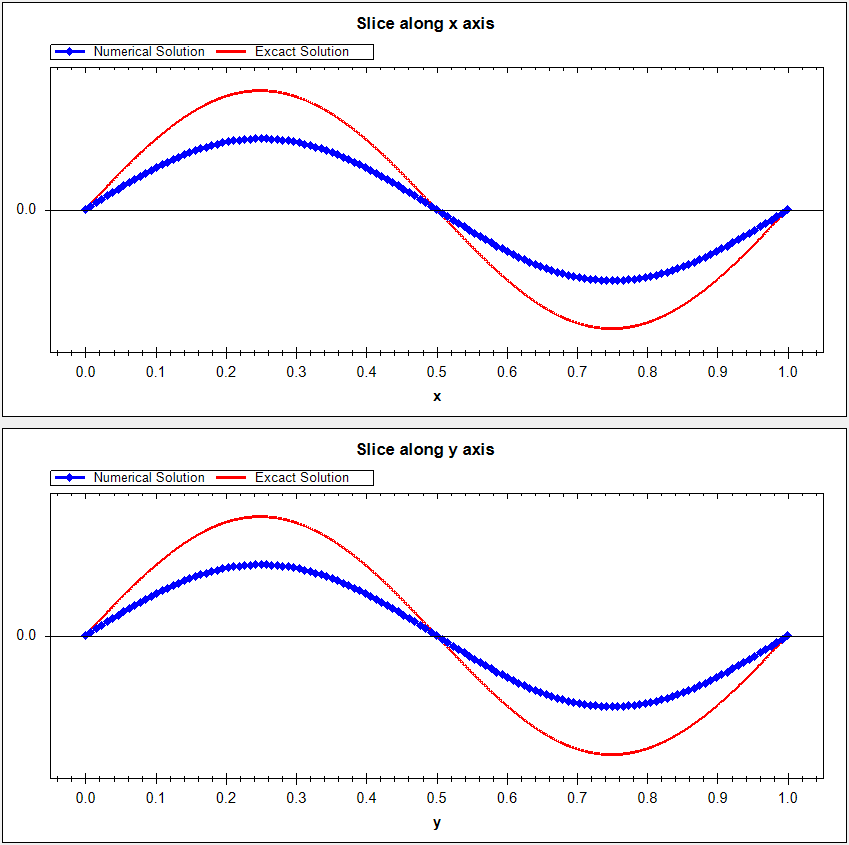
\includegraphics[width=0.45\textwidth]{../graphs/jacobi_129_0.001_750}}
    \hspace{3pt}
    \fbox{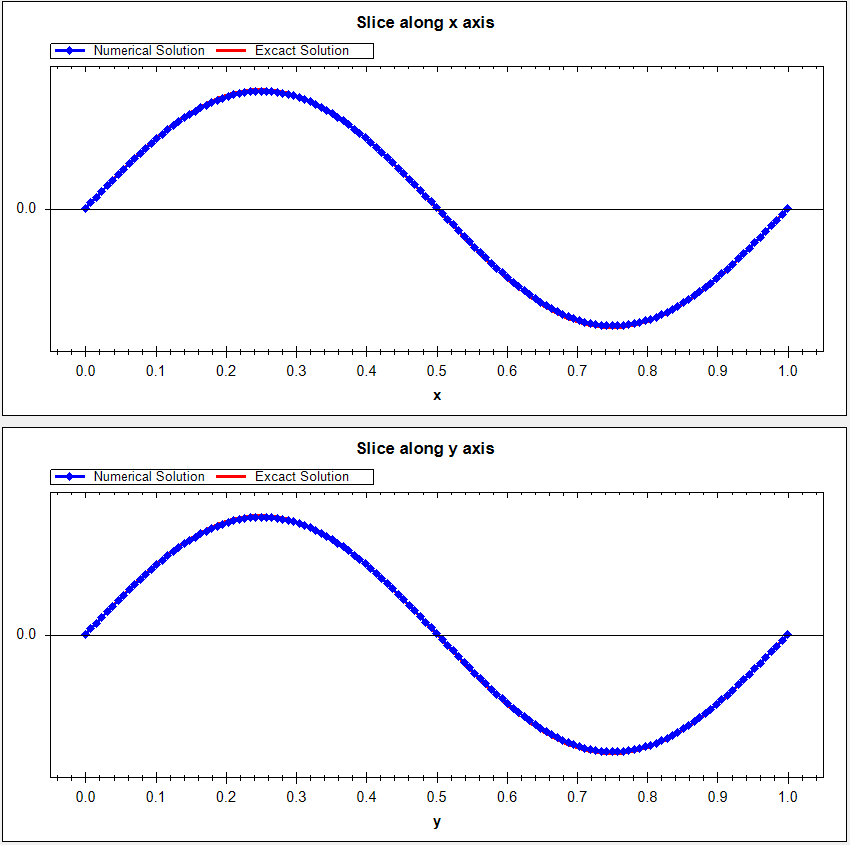
\includegraphics[width=0.45\textwidth]{../graphs/seidel_129_0.001_750}}
    \caption{Visual comparison of Jacobi and Seidel method graphs for $n=129$,
    750th iteration}
    \label{fig:vis2}
\end{figure}
\noindent
We can see that when it comes to visual proximity of the numerical solution to
the analytic solution Seidel's method is a lot more effective than Jacobi's
method.

\section{Conclusion}

Based on the features this report covered, I conclude that Seidel's method is
superior to Jacobi's method. Seidel's method generally requires fewer
iterations to reach a specific error threshold, it converges to the analytic
solution faster, and its visual proximity to the analytic solution increases
faster. Considering all of these factors, I think Seidel's method is better.\\
That does not mean, however, that Jacobi's method is bad. One big advantage of
this method compared to Seidel's method is that it converges consistently.
Seidel's method exhibits the "bounce" that can be seen in \figref{fig:err} but
Jacobi's method does not. This means that one can be sure that for a higher
number of iterations the accuracy will increase, while this is uncertain for
Seidel's method. In my opinion this does not make up for the 
disadvantages this method has compared to Seidel's method though.

\end{document}
